%-------------------------------------------------------------------------------
%-------------------------------------------------------------------------------
\begin{frame}
\begin{figure}[htp]\centering
\caption{Scientific Reading}
\scalebox{0.35}{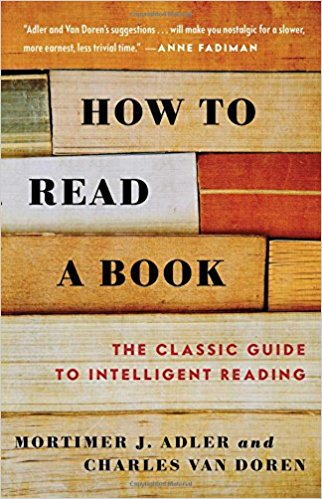
\includegraphics{fig-academic-reading-1}}
\end{figure}
\nocite{Adler.1972}
\end{frame}
%-------------------------------------------------------------------------------
%-------------------------------------------------------------------------------
\begin{frame}\textbf{Levels of reading}\vspace{0.3cm}
\begin{itemize}\setlength\itemsep{1em}
\item elementary
\item inspectional
\item analytical
\item syntopical
\end{itemize}
\end{frame}
%-------------------------------------------------------------------------------
%-------------------------------------------------------------------------------
\begin{frame}\textbf{Reading strategies}\vspace{0.3cm}
\begin{itemize}\setlength\itemsep{1em}
\item preview and skim\medskip
\begin{itemize}\setlength\itemsep{1em}
\item look for structural cues: headings, sub-headings, figures or images
\item look for context: where, when, who created the text
\item attempt to infer author's purpose and audience
\end{itemize}
\end{itemize}
\end{frame}
%-------------------------------------------------------------------------------
%-------------------------------------------------------------------------------
\begin{frame}
\begin{itemize}\setlength\itemsep{1em}
\item read actively\medskip
\begin{itemize}\setlength\itemsep{1em}
\item annotate the text with your questions
\item relate text to your own beliefs and experiences
\item identify new terms, concepts or sources to explore
\item note key points or conclusions
\end{itemize}
\end{itemize}
\end{frame}
%-------------------------------------------------------------------------------
%-------------------------------------------------------------------------------
\begin{frame}
\begin{itemize}\setlength\itemsep{1em}
\item outline and summarize\medskip
\begin{itemize}\setlength\itemsep{1em}
\item outline to see structure and flow of the text
\item summarize to check understanding
\item state main points and thesis for quick review
\end{itemize}
\end{itemize}
\end{frame}
%-------------------------------------------------------------------------------
%-------------------------------------------------------------------------------
\begin{frame}
\begin{itemize}\setlength\itemsep{1em}
\item question and wonder\medskip
\begin{itemize}\setlength\itemsep{1em}
\item how does the work contribute to your inquiry
\item how might the source help as evidence, background, and argument?
\item what evidence or persuasion does the author supply (fact, opinion, assumption)?
\item how does the text relate to other readings (contradict, support, extend)?
\end{itemize}
\end{itemize}

\end{frame}
%-------------------------------------------------------------------------------
%-------------------------------------------------------------------------------
\begin{frame}
\begin{itemize}
\item reread and reflect
\end{itemize}\vspace{0.5cm}
... see references for source\nocite{CUBoulder.2018}
\end{frame}
